\documentclass[onecolumn, draftclsnofoot,10pt, compsoc]{IEEEtran}
\usepackage{graphicx}
\usepackage{url}
\usepackage{setspace}
\usepackage{pstricks-add}
\usepackage{float}

\usepackage{geometry}
\geometry{textheight=9.5in, textwidth=7in}

% 1. Fill in these details
\def \CapstoneTeamName{		AKA Robotics}
\def \CapstoneTeamNumber{		13}
\def \GroupMemberOne{     Arthur Shing}
\def \GroupMemberTwo{			Kevin Talik}
\def \GroupMemberThree{   Anish Asrani}
\def \CapstoneProjectName{		How to Make an Effective Robot Comedian}
\def \CapstoneSponsorCompany{	Oregon State University}
\def \CapstoneSponsorPerson{		Heather Knight}

% 2. Uncomment the appropriate line below so that the document type works
\def \DocType{		%Problem Statement
				%Requirements Document
				%Technology Review
				Design Document
				%Progress Report
				}
			
\newcommand{\NameSigPair}[1]{\par
\makebox[2.75in][r]{#1} \hfil 	\makebox[3.25in]{\makebox[2.25in]{\hrulefill} \hfill		\makebox[.75in]{\hrulefill}}
\par\vspace{-12pt} \textit{\tiny\noindent
\makebox[2.75in]{} \hfil		\makebox[3.25in]{\makebox[2.25in][r]{Signature} \hfill	\makebox[.75in][r]{Date}}}}
% 3. If the document is not to be signed, uncomment the RENEWcommand below
\renewcommand{\NameSigPair}[1]{#1}

%%%%%%%%%%%%%%%%%%%%%%%%%%%%%%%%%%%%%%%
\begin{document}

\bstctlcite{IEEEexample:BSTcontrol}
\begin{titlepage}
    \pagenumbering{gobble}
    \begin{singlespace}
        \hfill 
        % 4. If you have a logo, use this includegraphics command to put it on the coversheet.
        %\includegraphics[height=4cm]{CompanyLogo}   
        \par\vspace{.2in}
        \centering
        \scshape{
            \huge CS Capstone \DocType \par
            {\large\today}\par
            \vspace{.5in}
            \textbf{\Huge\CapstoneProjectName}\par
            \vfill
            {\large Prepared for}\par
            \Huge \CapstoneSponsorCompany\par
            \vspace{5pt}
            {\Large\NameSigPair{\CapstoneSponsorPerson}\par}
            {\large Prepared by }\par
            Group\CapstoneTeamNumber\par
            % 5. comment out the line below this one if you do not wish to name your team
            \CapstoneTeamName\par 
            \vspace{5pt}
            {\Large
                \NameSigPair{\GroupMemberOne}\par
                \NameSigPair{\GroupMemberTwo}\par
                \NameSigPair{\GroupMemberThree}\par
            }
            \vspace{20pt}
        }
        \begin{abstract}
        \end{abstract}     
    \end{singlespace}
\end{titlepage}
\newpage
\pagenumbering{arabic}
\tableofcontents
% 7. uncomment this (if applicable). Consider adding a page break.
%\listoffigures
%\listoftables
\clearpage

% 8. now you write!
\section{Introduction}
  This is an intro

\section{Adaptation}
  We hypothesize that to make the set the most effective, the comedian needs to transition to topics; this is dependent on the audience response to jokes. The comedian will present an "initialization" procedure, known as the "Seed Jokes" to test the response of the audience to different jokes. Depending on their response, the comedian will transition to a theme that is evaluated to be the best fit. The robot comedian will have many jokes to choose from that contain different material, but not all audiences will like all of the jokes. Figure 1 shows how the theme will be chosen from a set of up to \textit{k} themes. The closing joke will be a subset of all jokes that might be stronger joke than some of the others, and is helpful in ending the show on a stronger note.

%\begin{figure}[H]
%  \centering
%  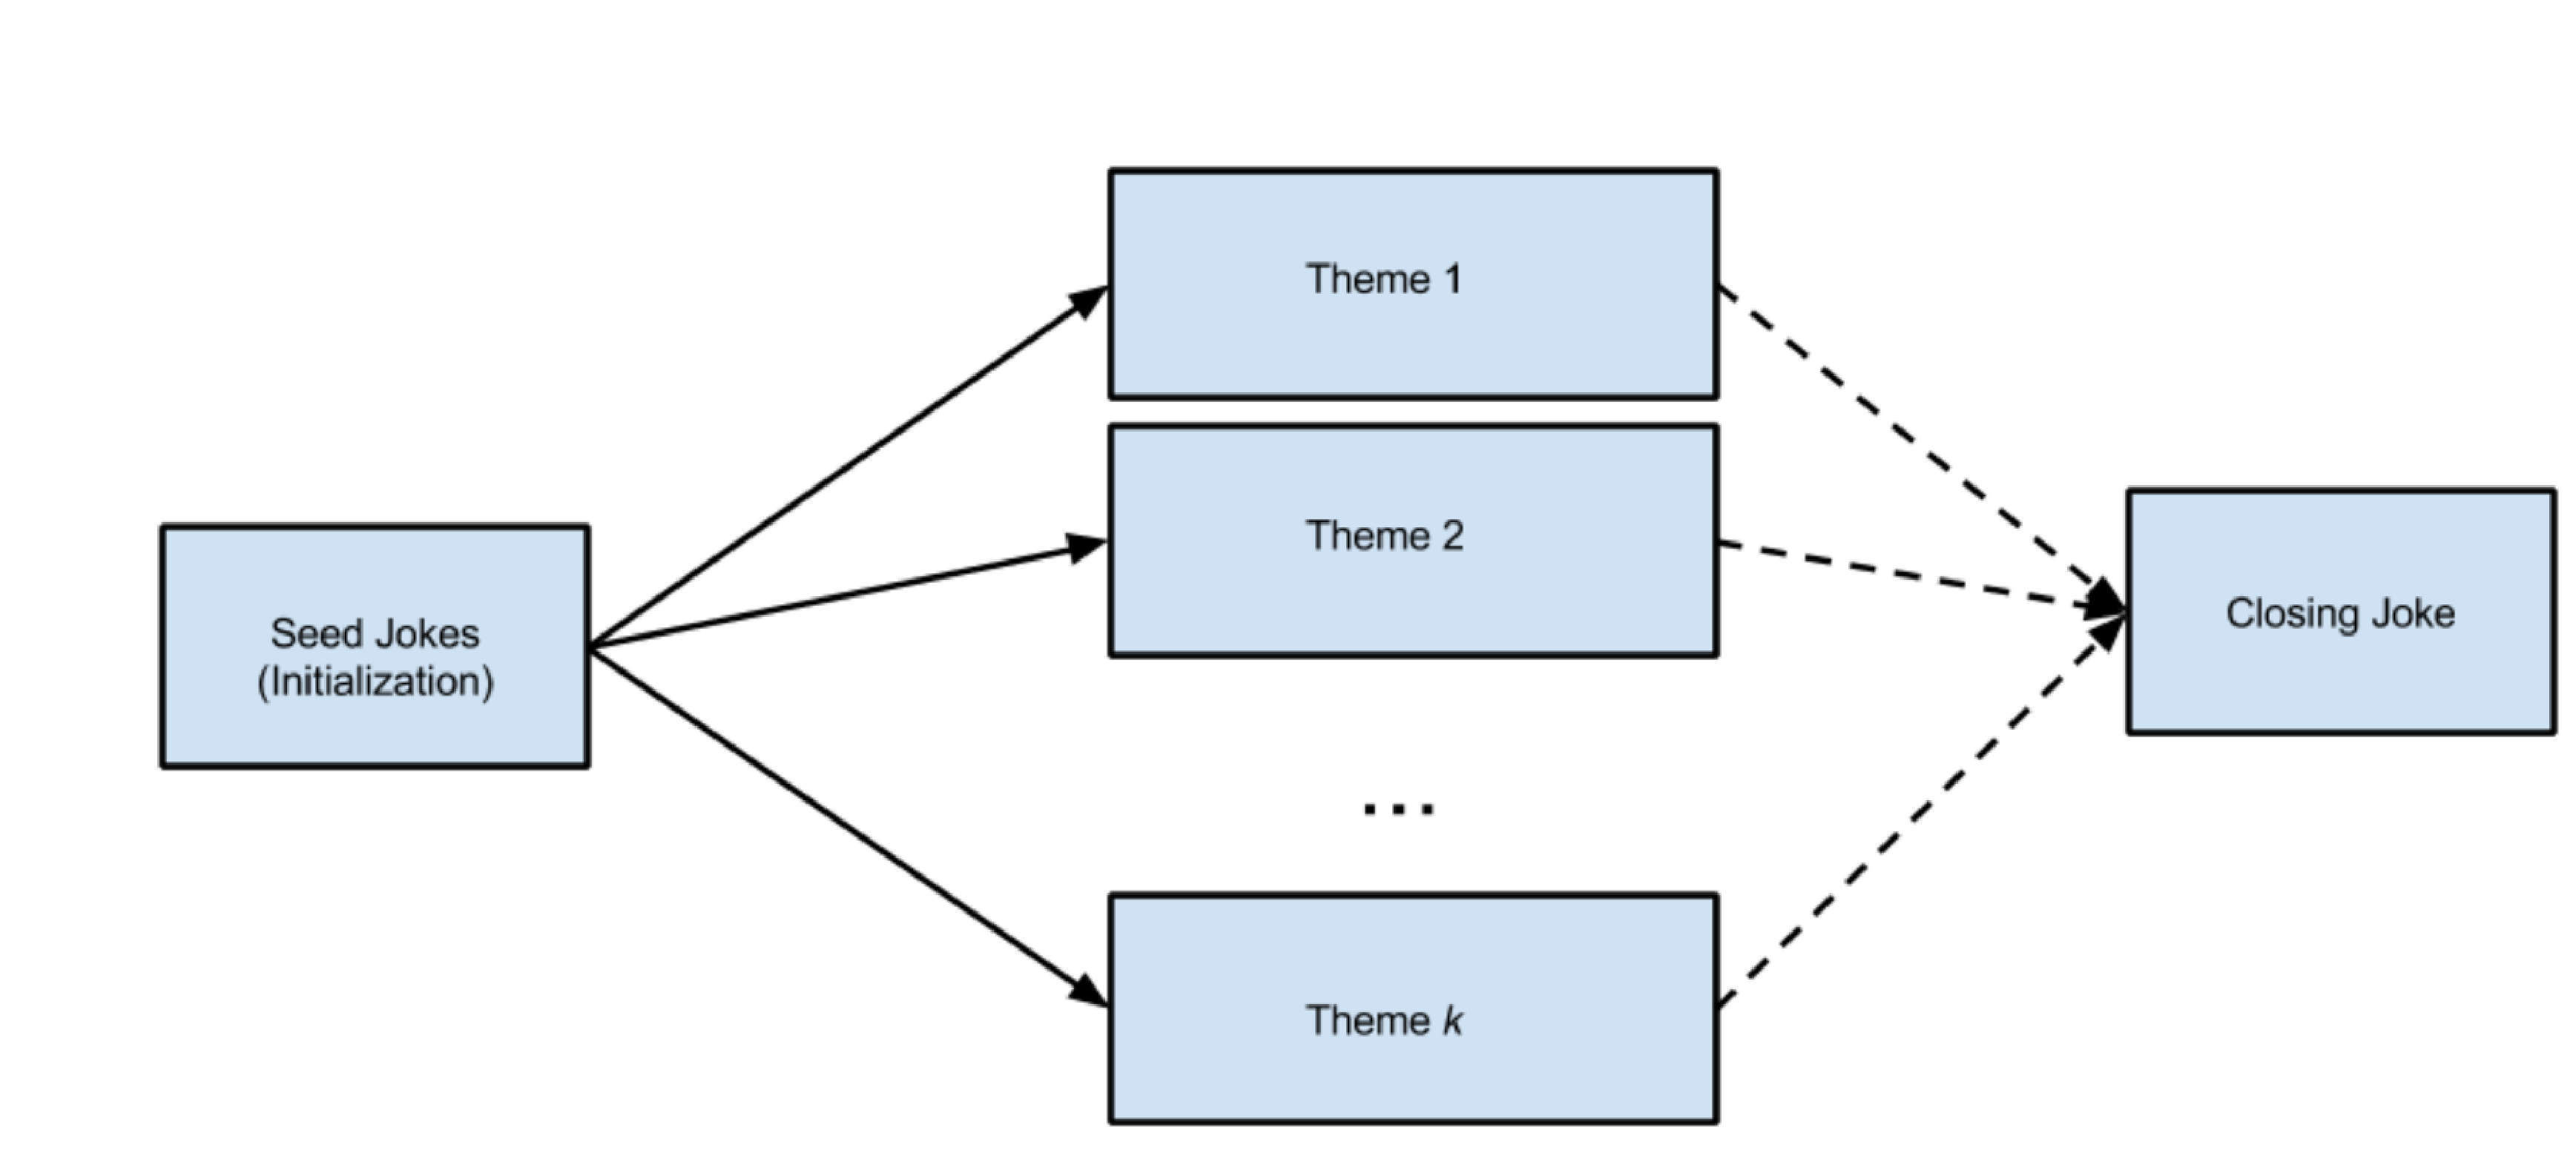
\includegraphics[width=0.5\textwidth,height=0.5\textheight]{fig0}
%\end{figure}

Figure 2 depicts how a joke will be interpreted by the robot. It will perform the joke, collect audience feedback information, then look up the jokes that will best fit the response. Further work needs to be done on heuristics for each joke, and matching that with audience feedback.
%\caption{Figure 1: Shows how algorithm will have up to \textit{k} Themes to choose from, determined from the seed joke. The closing joke is a subset of all jokes, and may be outside of a specific theme.}

\pagebreak


\bibliographystyle{IEEEtran}
\bibliography{refs}

\end{document}
